\documentclass{article}

\usepackage{graphicx}
\usepackage{tikz}
\usepackage{tikzsymbols}
\usetikzlibrary{calc,patterns,shapes.geometric}
\pagestyle{empty}
\usepackage[margin=0pt]{geometry}
\geometry{papersize={14in,12in}}

\def\centerarc[#1](#2)(#3:#4:#5){\draw[#1] ($(#2)+({#5*cos(#3)},{#5*sin(#3)})$) arc (#3:#4:#5);}

\begin{document}
	\begin{figure}
		\centering
		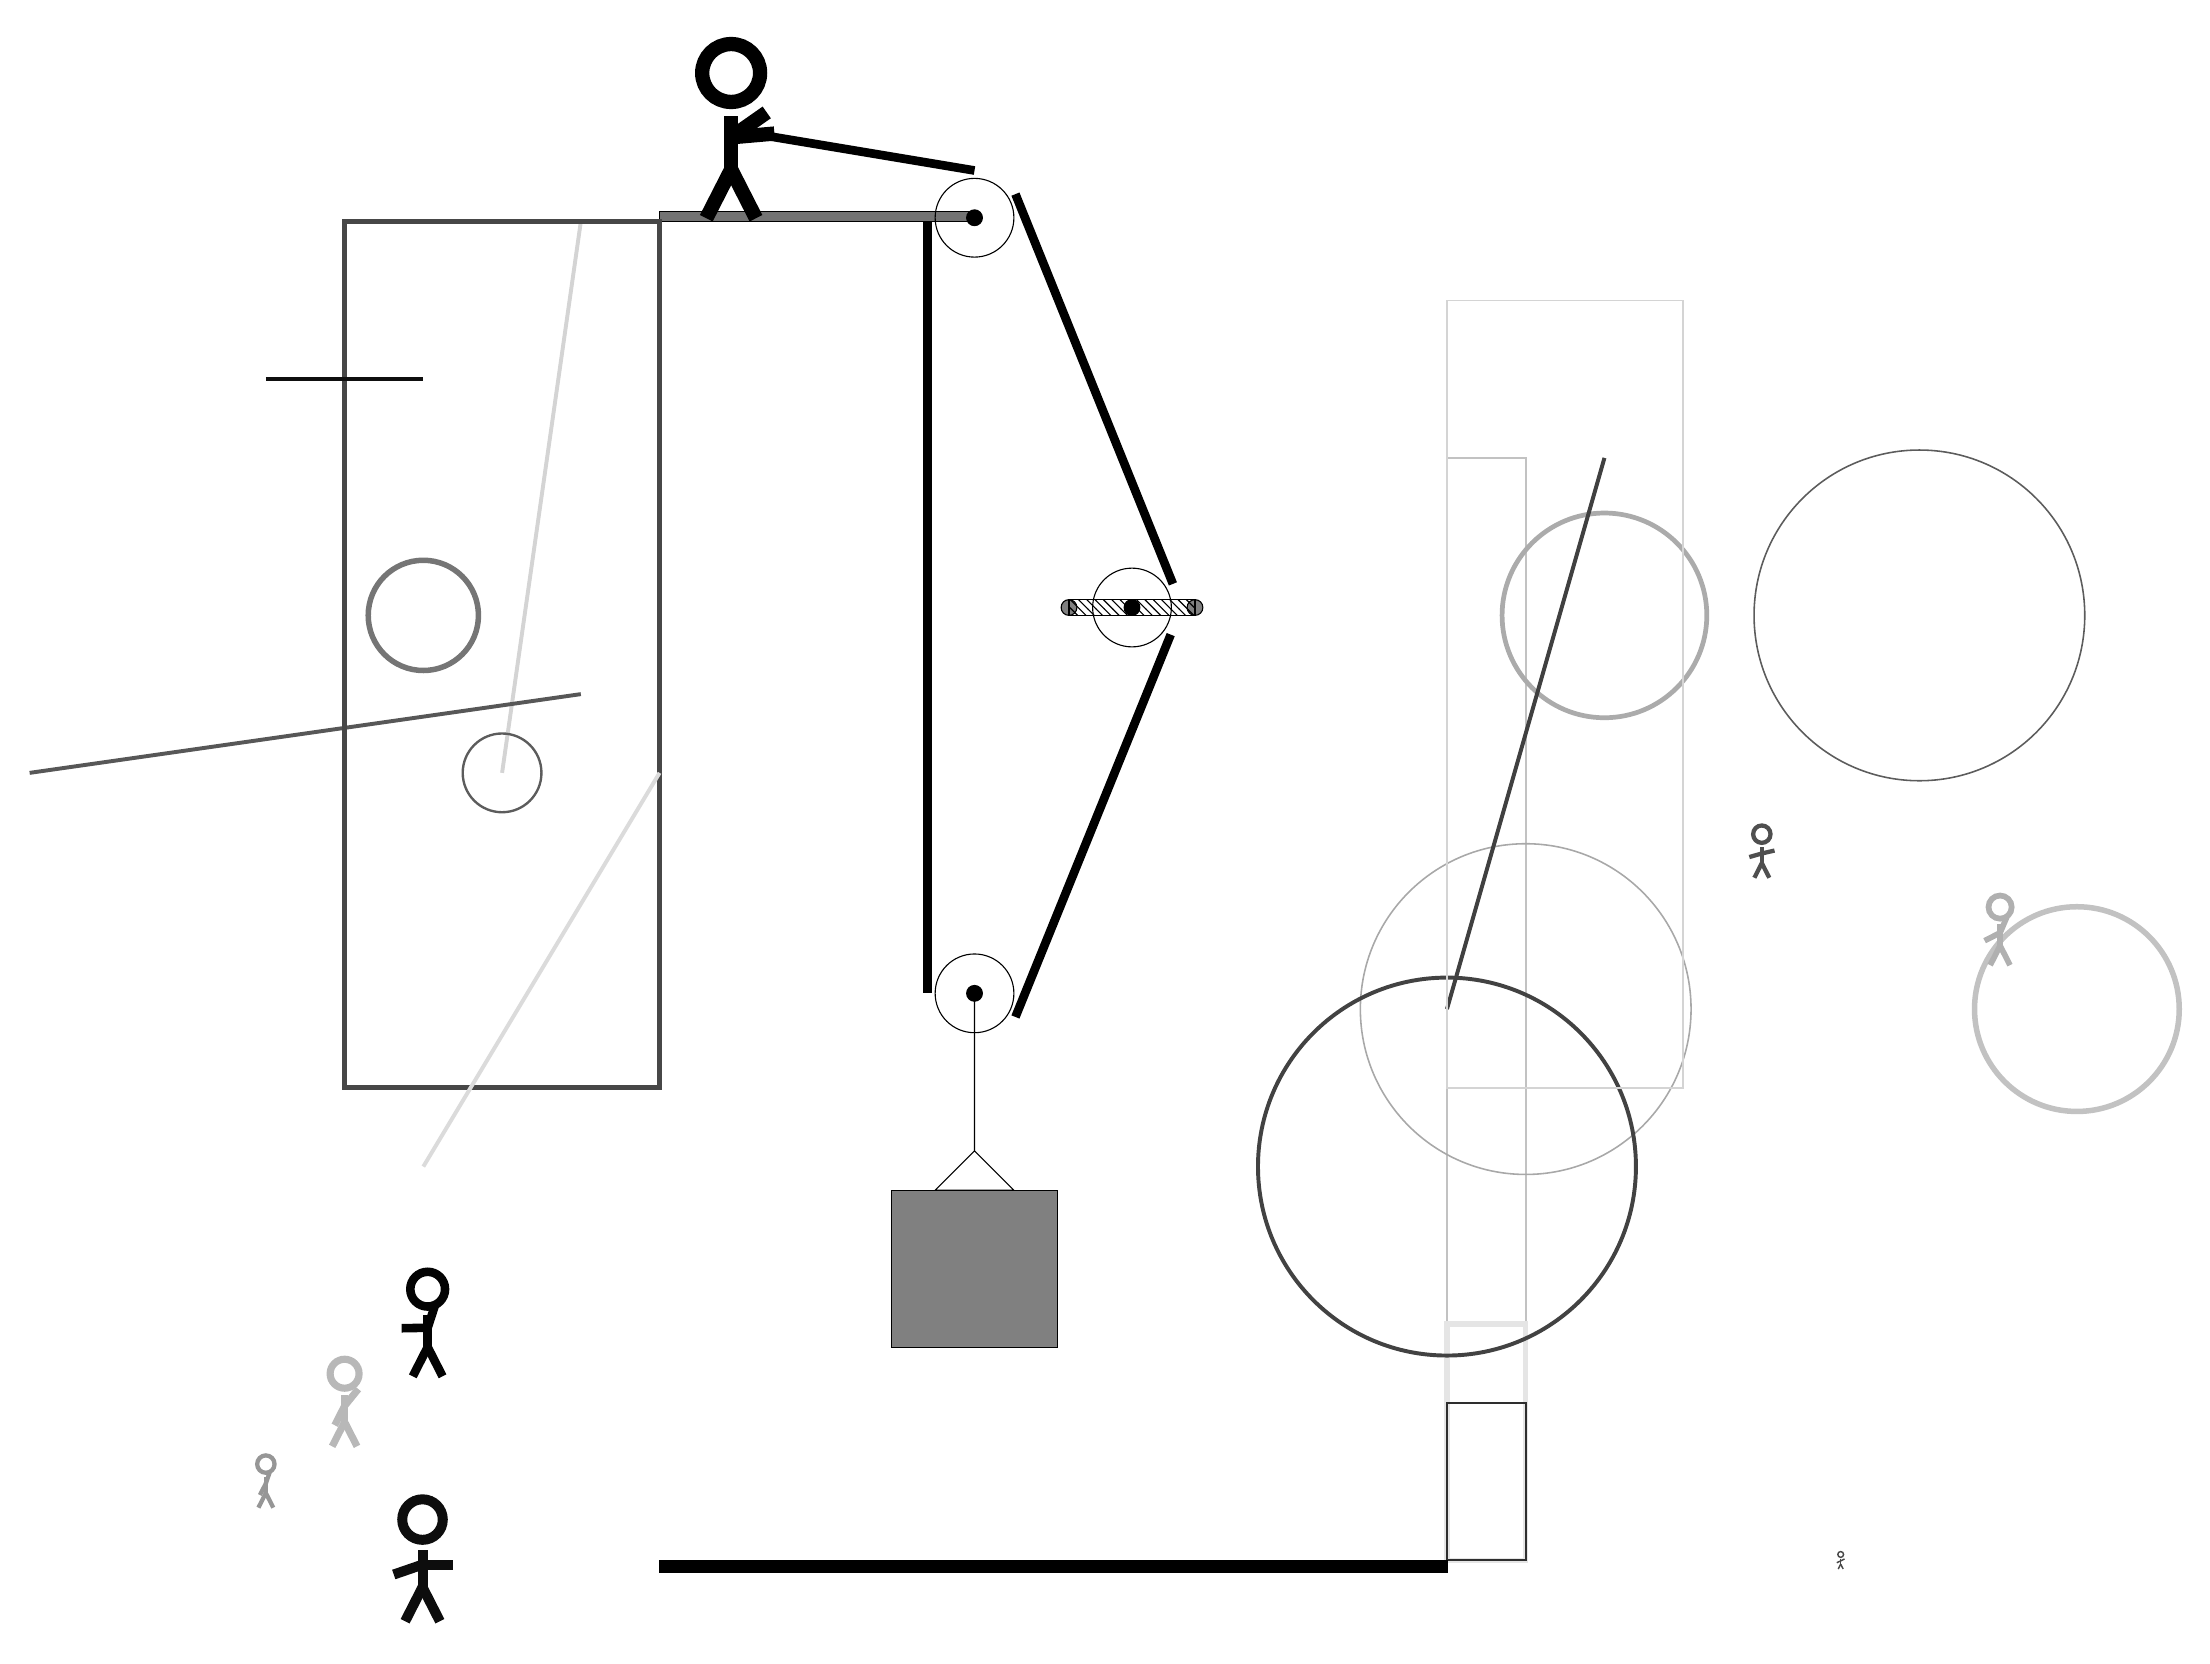
\begin{tikzpicture}
			%%%%% START %%%%%
			
			\draw[fill=black!55] (-2, 14) rectangle (2, 14.125);
			
			\draw (2, 4.2) circle (0.5);
			\draw[fill=black] (2, 4.2) circle (0.1);
			
			\draw (2, 14.05) circle (0.5);
			\draw[fill=black] (2, 14.05) circle (0.1);
			
			\draw[fill=white](4, 9.1) circle (0.5);
			\draw[fill=black] (4, 9.1) circle (0.1);
			\draw[fill=black!50] (3.2, 9.1) circle (0.1);
			\draw[fill=black!50] (4.8, 9.1) circle (0.1);
			\draw[pattern=north west lines, pattern color=black] (3.2, 9.2) rectangle (4.8, 9.0);
			
			\draw (2, 4.2) -- (2, 2.2) -- (1.5, 1.7) -- (2.5, 1.7) -- (2, 2.2);
			\draw[fill=black!50] (0.95, 1.7) rectangle (3.05, -0.3);
			
			\draw[line width=0.3mm, color=black!24] (8, 11) rectangle (9, 0);
			
			\draw [line width=0.7mm, color=black!24](16, 4) circle (1.3);
			\draw[line width=0.5mm, color=black!17](-3, 14) -- (-4, 7);
			\draw [line width=0.2mm, color=black!34](9, 4) circle (2.1);
			\node[line width=0.3mm, color=black!99] at (-5, 0) {\Strichmaxerl[6][1][72]};
			\draw[line width=0.7mm, color=black!10] (9, 0) rectangle (8, -3);
			
			\draw[line width=0.5mm, color=black!54] (-2, 13) rectangle (-2, 13);
			\draw[line width=0.5mm, color=black!66](-3, 8) -- (-10, 7);
			\node[line width=0.3mm, color=black!72] at (13, -3) {\Strichmaxerl[1][25][27]};
			\draw [line width=0.5mm, color=black!74](8, 2) circle (2.4);
			\draw[line width=0.2mm, color=black!82] (8, -1) rectangle (9, -3);
			\draw [line width=0.6mm, color=black!33](10, 9) circle (1.3);
			\draw[line width=0.5mm, color=black!75](8, 4) -- (10, 11);
			
			\node[line width=0.5mm, color=black!31] at (15, 5) {\Strichmaxerl[4][27][67]};
			\node[line width=0.3mm, color=black!95] at (-5, -3) {\Strichmaxerl[7][19][0]};
			\draw[line width=0.6mm, color=black!72] (-2, 14) rectangle (-6, 3);
			
			\node[line width=0.7mm, color=black!41] at (-7, -2) {\Strichmaxerl[3][63][71]};
			\node[line width=0.2mm, color=black!69] at (12, 6) {\Strichmaxerl[3][16][13]};
			\draw[line width=0.5mm, color=black!14](-5, 2) -- (-2, 7);
			\draw[line width=0.5mm, color=black!94](-7, 12) -- (-5, 12);
			\draw [line width=0.2mm, color=black!64](14, 9) circle (2.1);
			
			\draw[line width=0.2mm, color=black!17] (8, 3) rectangle (11, 13);
			\draw [line width=0.3mm, color=black!64](-4, 7) circle (0.5);
			\draw [line width=0.7mm, color=black!54](-5, 9) circle (0.7);
			\node[line width=0.3mm, color=black!28] at (-6, -1) {\Strichmaxerl[5][63][51]};
			
			\draw[line width=1.1mm] (1.4, 14) -- (1.4, 4.2);
			\centerarc[line width=1.1mm](2, 4.2)(180:330:0.6);
			\draw[line width=1.1mm](2.5196, 3.9) -- (4.4915, 8.7558);
			\centerarc[line width=1.1mm](4, 9.1)(390:325:0.6);
			\draw[line width=1.1mm](4.5196, 9.4) -- (2.5196, 14.35);
			\centerarc[line width=1.1mm](2, 14.05)(30:90:0.6);
			\draw[line width=1.1mm](2, 14.65) -- (-1, 15.15);
			
			\node at (-1, 15.15) {\Strichmaxerl[10][-175][35]};
			
			\draw[fill=black] (-2, -3) rectangle (8, -3.15);
			
			%%%%% END %%%%%
		\end{tikzpicture}
	\end{figure}	
\end{document}